\documentclass{beamer}

\usepackage[lined, ruled]{algorithm2e}
\usepackage{tikz}
\usepackage{enumitem}

\mode<presentation> {

% The Beamer class comes with a number of default slide themes
% which change the colors and layouts of slides. Below this is a list
% of all the themes, uncomment each in turn to see what they look like.

% \usetheme{default}
% \usetheme{AnnArbor}
% \usetheme{Antibes}
% \usetheme{Bergen}
% \usetheme{Berkeley}
\usetheme{Berlin} %<- this one is nice
% \usetheme{Boadilla} %  <- this one is nice
% \usetheme{CambridgeUS}
% \usetheme{Copenhagen}
% \usetheme{Darmstadt}
% \usetheme{Dresden}
% \usetheme{Frankfurt}
% \usetheme{Goettingen}
% \usetheme{Hannover}
% \usetheme{Ilmenau}
% \usetheme{JuanLesPins}
% \usetheme{Luebeck}
% \usetheme{Madrid} %<- this one is nice
% \usetheme{Malmoe}
% \usetheme{Marburg}
% \usetheme{Montpellier}
% \usetheme{PaloAlto}
% \usetheme{Pittsburgh}
% \usetheme{Rochester}
% \usetheme{Singapore}
% \usetheme{Szeged}
% \usetheme{Warsaw}

% As well as themes, the Beamer class has a number of color themes
% for any slide theme. Uncomment each of these in turn to see how it
% changes the colors of your current slide theme.

% \usecolortheme{albatross}
% \usecolortheme{beaver}
% \usecolortheme{beetle}
% \usecolortheme{crane} %<- this one is nice
\usecolortheme{dolphin} %<- this one is nice
% \usecolortheme{dove} %<- this one is nice
% \usecolortheme{fly}
% \usecolortheme{lily}
% \usecolortheme{orchid} %<- this one is nice
% \usecolortheme{rose} %<- this one is nice
% \usecolortheme{seagull} %<- this one is nice
% \usecolortheme{seahorse} %<- this one is nice
% \usecolortheme{whale} %<- this one is nice
% \usecolortheme{wolverine}

%\setbeamertemplate{footline} % To remove the footer line in all slides uncomment this line
\setbeamertemplate{footline}[page number] % To replace the footer line in all slides with a simple slide count uncomment this line
\setbeamertemplate{navigation symbols}{} % To remove the navigation symbols from the bottom of all slides uncomment this line
}


\title{Inverzije permutacij, permutacijski
grafi in tekmovalnostni grafi}
\author{Luka Uranič \\
\footnotesize{Mentorica: izr. prof. dr. Polona Oblak }}
\institute{Fakulteta za računalništvo in informatiko \\
Fakulteta za matematiko in fiziko}

\date{Ljubljana, 2023}

\begin{document}

\begin{frame}
\titlepage
\end{frame}

% \begin{frame}
% 	\tableofcontents
% \end{frame}
%%%%%%%%%%%%%%%%%%%%%%%%%%%%%%%%%%%%%%%%%%%%%
\section{Uvod}
\frame{
    \frametitle{Uvod}
    V delu smo si pogledali različne kombinatorične interpretacije inverzij permutacij. Za permutacijo smo predstavili njen graf inverzij in karakterizirali permutacijske grafe. Nato smo si ogledali tekmovalnostne grafe, ki so posplošitev permutacijskih grafov. Pokazali smo, kako jih lahko uporabimo za gručenje tekmovalcev.
}
%%%%%%%%%%%%%%%%%%%%%%%%%%%%%%%%%%%%%%%%%%%%%
\section{Permutacije in inverzije}
\frame{
    \frametitle{Permutacije in inverzije permutacij}
    \begin{block}{Definicija permutacije:}
        Bijektivni preslikavi $\pi: [n] \rightarrow [n]$ rečemo permutacija. 
    \end{block}
    Primer permutacije $\pi : [6] \rightarrow [6]$:
    \[
        \pi = \begin{pmatrix}
            1 & 2 & 3 & 4 & 5 & 6 \\
            3 & 1 & 5 & 2 & 6 & 4
        \end{pmatrix} = (3, 1, 5, 2, 6, 4).
    \]
    \begin{block}{Definicija inverzije:}
        Inverzija permutacije $\sigma = (a_1, a_2,\dots a_n) \in S_n$ je urejen par $(a_i, a_j)$, kjer je $i < j$ in $a_i > a_j$. 
    \end{block}
    Inverzije permutacije $\pi$ so $\{ (3, 1), (3, 2), (5, 2), (5, 4), (6, 4) \}$.
}
\frame{
    \frametitle{Število inverzij}   
    Število inverzij permutacije nam meri stopnjo neurejenosti oziroma oddaljenost permutacije od identične permutacije in je enako številu presečišč v puščičnem diagramu permutacije.
    
    \begin{figure}[ht]
        \begin{center}        
            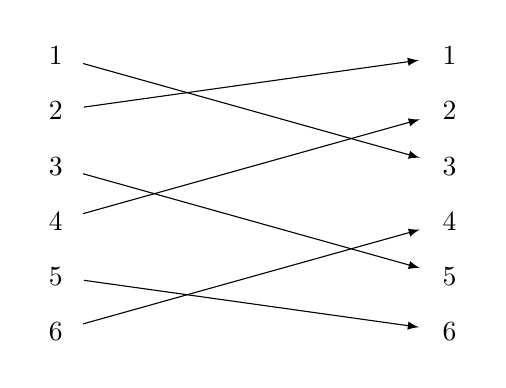
\begin{tikzpicture}[shorten >=1pt,-]
                \tikzstyle{vertex}=[circle,draw=black!0,fill=white!25,minimum size=20pt,inner sep=0pt]
                \foreach \num/\y in {1/.7, 2/1.4, 3/2.1, 4/2.8, 5/3.5, 6/4.2}
                    \node[vertex] (V-\num) at (0,5-\y) {$\num$};
                    \foreach \num/\y in {1/.7, 2/1.4, 3/2.1, 4/2.8, 5/3.5, 6/4.2}
                    \node[vertex] (VV-\num) at (5, 5-\y) {$\num$};
            
                \foreach \from/\to in {1/3, 2/1, 3/5, 4/2, 5/6, 6/4}
                    \draw[-latex] (V-\from) -- (VV-\to);
            \end{tikzpicture}     
        \end{center}
        \label{bijektivna_preslikava_n_n}
    \end{figure}
    Identična permutacija $id = (1, 2, \dots, n)$ nima inverzij.\\
    Permutacija $(n, n-1, \dots, 1)$ ima $\binom{n}{2}$ inverzij.
}
% \frame{
%     \frametitle{Šibka Bruhatova delna urejenost}    
%     \begin{block}{Definicija šibke Bruhatove delne urejenosti:}
%         Naj bosta $\sigma, \pi \in S_n$. Permutacija $\sigma$ je manjša ali enaka od permutacije $\pi$ v šibki Bruhatovi delni urejenosti, kar označimo z $\sigma \preceq_b \pi$, če je $I_{\sigma} \subseteq I_{\pi}$. 
%     \end{block}
% }
% \frame{
% \begin{figure}[h]
%     \begin{center}        
%         \begin{tikzpicture}[shorten >=1pt,-]
%             \tikzstyle{vertex}=[circle,draw=black!0,fill=white!25,minimum size=20pt,inner sep=0pt]
%             \foreach \num/\x in {1234/2.5}
%                 \node[vertex] (V-\num) at (\x, 0) {$\num$};
%             \foreach \num/\x in {1243/1.5, 1324/2.5, 2134/3.5}
%                 \node[vertex] (V-\num) at (\x, 1) {$\num$};                
%             \foreach \num/\x in {1423/0.5, 1342/1.5, 2143/2.5, 3124/3.5, 2314/4.5}
%                 \node[vertex] (V-\num) at (\x, 2) {$\num$};
%             \foreach \num/\x in {1432/0, 4123/1, 2413/2, 3142/3, 3214/4, 2341/5}
%                 \node[vertex] (V-\num) at (\x, 3) {$\num$};                
%             \foreach \num/\x in {4132/0.5, 4213/1.5, 3412/2.5, 2431/3.5, 3241/4.5}
%                 \node[vertex] (V-\num) at (\x, 4) {$\num$};            
%             \foreach \num/\x in {4312/1.5, 4231/2.5, 3421/3.5}
%                 \node[vertex] (V-\num) at (\x, 5) {$\num$};
%             \foreach \num/\x in {4321/2.5}
%                 \node[vertex] (V-\num) at (\x, 6) {$\num$};

%             \foreach \from/\to in {1234/1243, 1234/1324, 1234/2134, 1243/1423, 1243/2143, 1324/1342, 1324/3124, 2134/2143, 2134/2314, 1423/1432, 1423/4123, 1342/1432, 1342/3142, 2143/2413, 3124/3142, 3124/3214, 2314/3214, 2314/2341, 1432/4132, 4123/4132, 4123/4213, 2413/4213, 2413/2431, 3142/3412, 3214/3241, 2341/2431, 2341/3241, 4132/4312, 4213/4231, 3412/4312, 3412/3421, 2431/4231, 3241/3421, 4312/4321, 4231/4321, 3421/4321}
%                 \draw (V-\from) -- (V-\to);
%         \end{tikzpicture}     
%     \end{center}
%     \caption{Hessejev diagram šibke Bruhatove delne urejenosti množice $S_4$.}
%     \label{sibka_bruhatova_urejenost_S4}
% \end{figure}
% }
% \frame{
%     \frametitle{Rodovne funkcije permutacij}
%     Naj bo $f_n(x)$ rodovna funkcija s koeficienti $a_i$ pred $x^i$, ki štejejo število permutacij množice $[n]$ z $i$ inverzijami:
%     \[
%         f_n(x) = \sum_{i=0}^{\binom{n}{2}} a_i x^i.
%     \]
%     Število vseh permutacij množice $[n]$ je $n!$, zato velja:
%     \[
%         \sum_{i=0}^{\binom{n}{2}} a_i = n!.
%     \]
% }
% \frame{
%     \frametitle{Rodovne funkcije permutacij}
%     Eksplicitna formula za rodovno funkcijo:
%     \[
%         f_n(x) = \prod_{m=1}^{n}\sum_{i=0}^{m-1} x^i = 1 (1 + x) (1 + x + x^2) \cdot\cdot\cdot (1 + x + \cdot\cdot\cdot + x^{n-1}).
%     \]
%     Naslednja formula nam pove, kako iz rodovne funkcije $f_n$ izrazimo koeficient $a_i$:
%     \[
%         a_i = \binom{n\!+\!i\!-\!1}{i} + \sum_{j=1}^{\infty} (-1)^j \left( \binom{n\!+\!i\!-\!u_j\!-\!j\!-\!1}{i\!-\!u_j\!-\!j} + \binom{n\!+\!i\!-\!u_j\!-\!1}{i\!-\!u_j} \right),
%     \]
%     kjer so $u_j = \frac{j(3j-1)}{2}$ petkotniška števila. Če je v binomskem simbolu spodaj negativno število, je vrednost binomskega simbola enaka $0$. Zato je vsota končna.
% }
%%%%%%%%%%%%%%%%%%%%%%%%%%%%%%%%%%%%%%%%%%%%%
\section{Permutacijski grafi}
\frame{
    \frametitle{Permutacijski grafi}    
    \begin{block}{Definicija permutacijskega grafa:}
        Naj bo $\sigma \in S_n$. Graf inverzij permutacije $\sigma$, ki ga označimo z $G_{\sigma}$, je neusmerjen graf z $V(G_{\sigma}) = [n]$, kjer je $xy \in E(G_{\sigma})$ natanko tedaj, ko je $(x, y)$ ali $(y, x)$ inverzija permutacije $\sigma$. Vsak graf izomorfen grafu $G_{\sigma}$ za neko permutacijo $\sigma$ imenujemo permutacijski graf.
    \end{block}
    
    \begin{figure}[h]
        \begin{center}        
            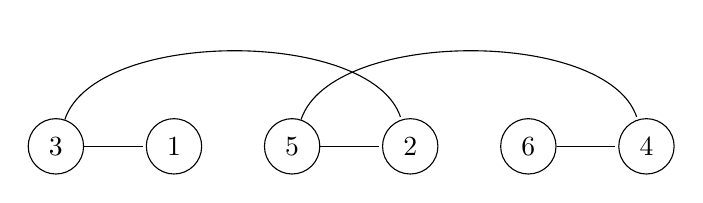
\begin{tikzpicture}[shorten >=1pt,-]
                \tikzstyle{vertex}=[circle,draw=black,fill=white!25,minimum size=20pt,inner sep=0pt]
                \foreach \num/\x in {3/1, 1/2.5, 5/4, 2/5.5, 6/7, 4/8.5}
                        \node[vertex] (V-\num) at (\x,0) {$\num$};
                        
                    \foreach \from/\to in {3/1, 5/2, 6/4}
                        \draw (V-\from) -- (V-\to);
            
                    \draw (V-3) .. controls (1.5, 1.5) and (5, 1.5) .. (V-2);
                    \draw (V-5) .. controls (4.5, 1.5) and (8, 1.5) .. (V-4);
                    
            \end{tikzpicture}     
        \end{center}
        \label{graf_permutacijski_graf}
    \end{figure}
}
\frame{
    \frametitle{Kohezivno zaporedje grafa}    
    \begin{block}{Definicija kohezivnega zaporedja grafa:}
        Naj bo $G$ neusmerjen graf na $n$ vozliščih. 
        Zaporedju vozlišč $l = (v_1, v_2, \dots, v_n)$ rečemo kohezivno zaporedje grafa $G$, če sta za poljubne $i, j, k$, kjer je $1 \leq i < k < j \leq n$, izpolnjena naslednja pogoja:
        \begin{enumerate}[label=(\alph*)]
            \item Če je $v_iv_k \in E(G)$, $v_kv_j \in E(G)$, potem je $v_iv_j \in E(G)$.
            \item Če je $v_iv_j \in E(G)$, potem je $v_iv_k \in E(G)$ ali $v_kv_j \in E(G)$.
        \end{enumerate}
    \end{block}
    
    \begin{figure}[h]
        \begin{center}        
            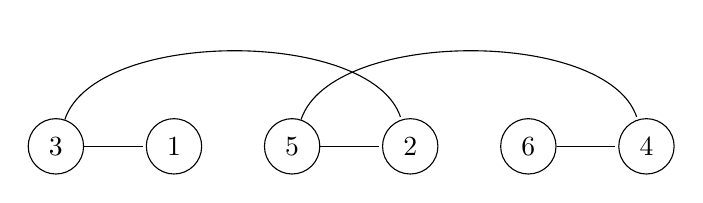
\begin{tikzpicture}[shorten >=1pt,-]
                \tikzstyle{vertex}=[circle,draw=black,fill=white!25,minimum size=20pt,inner sep=0pt]
                \foreach \num/\x in {3/1, 1/2.5, 5/4, 2/5.5, 6/7, 4/8.5}
                        \node[vertex] (V-\num) at (\x,0) {$\num$};
                        
                    \foreach \from/\to in {3/1, 5/2, 6/4}
                        \draw (V-\from) -- (V-\to);
            
                    \draw (V-3) .. controls (1.5, 1.5) and (5, 1.5) .. (V-2);
                    \draw (V-5) .. controls (4.5, 1.5) and (8, 1.5) .. (V-4);
                    
            \end{tikzpicture}     
        \end{center}
        \label{graf_permutacijski_graf2}
    \end{figure}
}
\frame{
    \frametitle{Karakterizacija permutacijskih grafov}    
    % \begin{block}{Lema:}
    %     Naj bo $G$ graf. Zaporedje vozlišč $l$ je kohezivno zaporedje grafa $G$ natanko tedaj, ko je $l$ kohezivno zaporedje grafa $\overline{G}$. 
    % \end{block}
    \begin{block}{Izrek:}
        Naj bo $\sigma \in S_n$. Zaporedje vozlišč $(\sigma(1), \sigma(2), \dots, \sigma(n))$ je kohezivno zaporedje permutacijskega grafa $G_{\sigma}$.
    \end{block}
    \begin{block}{Izrek (karakterizacija permutacijskih grafov):}
        Graf $G$ je permutacijski graf natanko tedaj, ko ima kohezivno zaporedje.
    \end{block}
}
\frame{
    \frametitle{Zvezde in poti}    
    \begin{block}{Trditev:}
        Zvezda $K_{1,n}$ je permutacijski graf.
    \end{block}
    \begin{figure}[h]
        \begin{center}        
            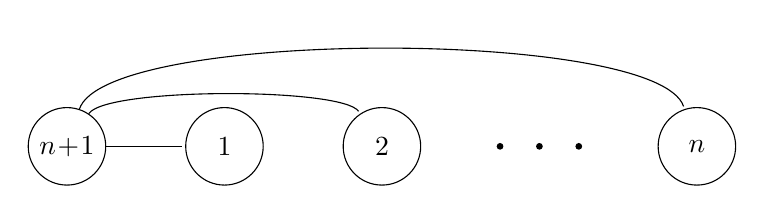
\begin{tikzpicture}[shorten >=1pt,-]
                \tikzstyle{vertex}=[circle,draw=black,fill=white!25,minimum size=28pt,inner sep=0pt]
                \foreach \num/\x in {1/3, 2/5, n/9}
                        \node[vertex] (V-\num) at (\x,0) {$\num$};
                        
                    \node[vertex] (V-n+1) at (1,0) {$n\!+\!1$};
                    \foreach \from/\to in {n+1/1}
                        \draw (V-\from) -- (V-\to);
    
                    \draw (V-n+1) .. controls (1.5, 0.75) and (4.5, 0.75) .. (V-2);
                    \draw (V-n+1) .. controls (1.5, 1.5) and (8.5, 1.5) .. (V-n);
    
                    
                    \filldraw [black] (6.5,0) circle (1pt);
                    \filldraw [black] (7,0) circle (1pt);
                    \filldraw [black] (7.5,0) circle (1pt);
            \end{tikzpicture} 
        \end{center}
        \label{graf_kohezivnega_zaporedja_zvezda}
    \end{figure}
    \begin{block}{Trditev:}
        Pot $P_n$ je permutacijski graf.
    \end{block}
    \begin{figure}[h]
        \begin{center}        
            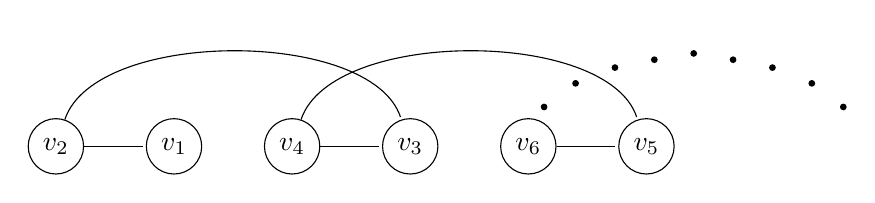
\begin{tikzpicture}[shorten >=1pt,-]
                \tikzstyle{vertex}=[circle,draw=black,fill=white!25,minimum size=20pt,inner sep=0pt]
                \foreach \num/\x in {v_2/1, v_1/2.5, v_4/4, v_3/5.5, v_6/7, v_5/8.5}
                        \node[vertex] (V-\num) at (\x,0) {$\num$};
                        
                    \foreach \from/\to in {v_2/v_1, v_4/v_3, v_6/v_5}
                        \draw (V-\from) -- (V-\to);
            
                    \draw (V-v_2) .. controls (1.5, 1.5) and (5, 1.5) .. (V-v_3);
                    \draw (V-v_4) .. controls (4.5, 1.5) and (8, 1.5) .. (V-v_5);
                    
                    \filldraw [black] (7.2,0.5) circle (1pt);
                    \filldraw [black] (7.6,0.8) circle (1pt);
                    \filldraw [black] (8.1,1) circle (1pt);
                    \filldraw [black] (8.6,1.1) circle (1pt);
                    \filldraw [black] (9.1,1.18) circle (1pt);
                    \filldraw [black] (9.6,1.1) circle (1pt);
                    \filldraw [black] (10.1,1) circle (1pt);
                    \filldraw [black] (10.6,0.8) circle (1pt);
                    \filldraw [black] (11,0.5) circle (1pt);
            \end{tikzpicture}     
        \end{center}
        \label{graf_kohezivnega_zaporedja_pot}
    \end{figure}
}
\frame{
    \frametitle{Drevo $K_{1,3}^*$}
    \begin{block}{Trditev:}
        Drevo $K_{1,3}^*$ ni permutacijski graf.
    \end{block}
    \begin{figure}[h]
        \begin{center}        
            \begin{tikzpicture}[shorten >=1pt,-]
                \tikzstyle{vertex}=[circle,draw=black,fill=white!25,minimum size=20pt,inner sep=0pt]
                        \node[vertex] (V-0) at (4,4){};
                        \node[vertex] (V-1) at (4,1.75){};
                        \node[vertex] (V-2) at (2,0){};
                        \node[vertex] (V-3) at (6,0){};
            
                    \foreach \from/\to in {0/1, 1/2, 1/3}
                        \draw (V-\from) -- (V-\to);
            \end{tikzpicture}\qquad
            \begin{tikzpicture}[shorten >=1pt,-]
                \tikzstyle{vertex}=[circle,draw=black,fill=white!25,minimum size=20pt,inner sep=0pt]
                        \node[vertex] (V-0) at (4,4){};
                        \node[vertex] (V-01) at (4,2.90){};
                        \node[vertex] (V-1) at (4,1.75){};
                        \node[vertex] (V-12) at (3, 0.875){};
                        \node[vertex] (V-2) at (2,0){};
                        \node[vertex] (V-13) at (5,0.875){};
                        \node[vertex] (V-3) at (6,0){};
            
                    \foreach \from/\to in {0/01, 12/2, 13/3, 01/1, 1/12, 1/13}
                        \draw (V-\from) -- (V-\to);
            \end{tikzpicture}
        \end{center}
        \label{graf_subdivizija_k13}
    \end{figure}    
}
\frame{
    \frametitle{Gosenice}    
    \begin{block}{Definicija gosenice:}
        Drevo je gosenica, če po odstranitvi vseh listov dobimo pot.
    \end{block}
    \begin{block}{Lema:}
        Drevo je gosenica natanko tedaj, ko ne vsebuje podgrafa $K_{1,3}^*$.
    \end{block}
    \begin{figure}[h]
        \begin{center}        
            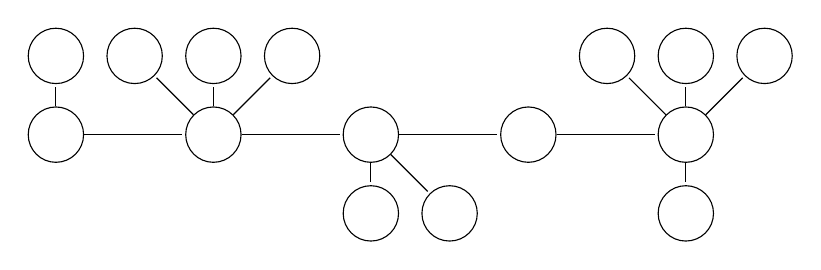
\begin{tikzpicture}[shorten >=1pt,-]
                \tikzstyle{vertex}=[circle,draw=black,fill=white!25,minimum size=20pt,inner sep=0pt]
                        \node[vertex] (V-0) at (0, 1){};
                        \node[vertex] (V-1) at (2, 1){};
                        \node[vertex] (V-2) at (4, 1){};
                        \node[vertex] (V-3) at (6, 1){};
                        \node[vertex] (V-4) at (8, 1){};
                        \node[vertex] (V-5) at (0, 2){};
                        \node[vertex] (V-6) at (2, 2){};
                        \node[vertex] (V-7) at (1, 2){};
                        \node[vertex] (V-8) at (3, 2){};
                        \node[vertex] (V-9) at (4, 0){};
                        \node[vertex] (V-10) at (5, 0){};
                        \node[vertex] (V-11) at (8, 0){};
                        \node[vertex] (V-12) at (7, 2){};
                        \node[vertex] (V-13) at (8, 2){};
                        \node[vertex] (V-14) at (9, 2){};
            
                    \foreach \from/\to in {0/1, 1/2, 2/3, 3/4, 0/5, 1/6, 1/7, 1/8, 2/9, 2/10, 4/11, 4/12, 4/13, 4/14}
                        \draw (V-\from) -- (V-\to);
            \end{tikzpicture}
        \end{center}
        \label{graf_gosenice_10_listov}
    \end{figure}
}
\frame{
    \frametitle{Drevesa, ki so permutacijski grafi}
    \begin{block}{Izrek:}
        Drevo je permutacijski graf natanko tedaj, ko je gosenica.
    \end{block}
    \begin{figure}[h]
        \begin{center}        
            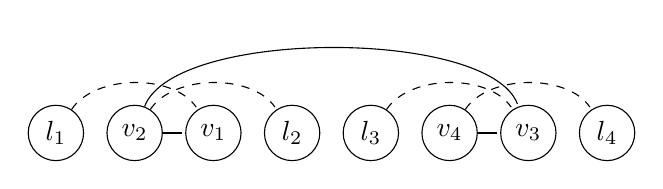
\begin{tikzpicture}[shorten >=1pt,-]
                \tikzstyle{vertex}=[circle,draw=black,fill=white!25,minimum size=20pt,inner sep=0pt]
                \foreach \num/\x in {l_1/0, v_2/1, v_1/2, l_2/3, l_3/4, v_4/5, v_3/6, l_4/7}
                        \node[vertex] (V-\num) at (\x,0) {$\num$};
            
                    \foreach \from/\to in {v_2/v_1, v_4/v_3}
                        \draw (V-\from) -- (V-\to);
            
                    \draw[dashed] (V-l_1) .. controls (0.5, 0.75) and (1.5, 0.75) .. (V-v_1);
                    \draw[dashed] (V-l_3) .. controls (4.5, 0.75) and (5.5, 0.75) .. (V-v_3);
        
                    \draw[dashed] (V-v_2) .. controls (1.5, 0.75) and (2.5, 0.75) .. (V-l_2);
                    \draw[dashed] (V-v_4) .. controls (5.5, 0.75) and (6.5, 0.75) .. (V-l_4);
                    
                    \draw (V-v_2) .. controls (1.5, 1.33) and (5.5, 1.33) .. (V-v_3);
                    
            \end{tikzpicture}
        \end{center}
        \label{graf_kohezivnega_zaporedja_gosenice}
    \end{figure}
}
% \frame{
%     \frametitle{Permutacije gosenic}
%     \begin{block}{Trditev:}
%         Vsaka gosenica $C$ je permutacijski graf vsaj dveh permutacij.
%     \end{block}
    
%     \begin{figure}[h]
%         \begin{center}        
%             \begin{tikzpicture}[shorten >=1pt,-]
%                 \tikzstyle{vertex}=[circle,draw=black,fill=white!25,minimum size=20pt,inner sep=0pt]
%                 \tikzstyle{vertex2}=[circle,draw=black!,fill=black!10,minimum size=20pt,inner sep=0pt]
%                 \foreach \num/\x in {5/1, 1/2, 8/5, 4/6}
%                         \node[vertex] (V-\num) at (\x,0) {$\num$};
%                 \foreach \num/\x in {2/0, 3/3, 6/4, 7/7}
%                         \node[vertex2] (V-\num) at (\x,0) {$\num$};
            
%                     \foreach \from/\to in {5/1, 8/4}
%                         \draw (V-\from) -- (V-\to);
            
%                     \draw (V-2) .. controls (0.5, 0.75) and (1.5, 0.75) .. (V-1);
%                     \draw (V-6) .. controls (4.5, 0.75) and (5.5, 0.75) .. (V-4);
        
%                     \draw (V-5) .. controls (1.5, 0.75) and (2.5, 0.75) .. (V-3);
%                     \draw (V-8) .. controls (5.5, 0.75) and (6.5, 0.75) .. (V-7);
%                     \draw (V-5) .. controls (1.5, 1.33) and (5.5, 1.33) .. (V-4);
%             \end{tikzpicture}\\\quad\\                    
%             \begin{tikzpicture}[shorten >=1pt,-]
%                 \tikzstyle{vertex}=[circle,draw=black,fill=white!25,minimum size=20pt,inner sep=0pt]
%                 \tikzstyle{vertex2}=[circle,draw=black!,fill=black!10,minimum size=20pt,inner sep=0pt]
%                 \foreach \num/\x in {3/0, 7/3, 2/4, 6/7}
%                         \node[vertex] (V-\num) at (\x,0) {$\num$};
%                 \foreach \num/\x in {1/1, 4/2, 5/5, 8/6}
%                         \node[vertex2] (V-\num) at (\x,0) {$\num$};
            
%                     \foreach \from/\to in {3/1, 7/2, 8/6}
%                         \draw (V-\from) -- (V-\to);
            
%                     \draw (V-4) .. controls (2.5, 0.75) and (3.5, 0.75) .. (V-2);
%                     \draw (V-7) .. controls (3.5, 0.75) and (4.5, 0.75) .. (V-5);
    
%                     \draw (V-3) .. controls (0.5, 1.1) and (3.5, 1.1) .. (V-2);
%                     \draw (V-7) .. controls (3.5, 1.1) and (6.5, 1.1) .. (V-6);
%             \end{tikzpicture}
%         \end{center}
%         \label{tranzitivni_orientaciji_gosenice}
%     \end{figure}
% }
\frame{
    \frametitle{Permutacije gosenic}
    % \begin{block}{Izrek:}
    %     Za $n \geq 3$ obstajata natanko dve permutaciji iz $S_n$, katerih permutacijski graf je pot na $n$ vozliščih.
    % \end{block}
    \begin{block}{Izrek:}
        Naj bo $n \geq 3$ in $C$ gosenica na $n$ vozliščih. Potem obstajata natanko dve permutaciji iz $S_n$, katerih permutacijski graf je izomorfen grafu gosenice $C$.
    \end{block}
    \begin{figure}[h]
        \begin{center}        
            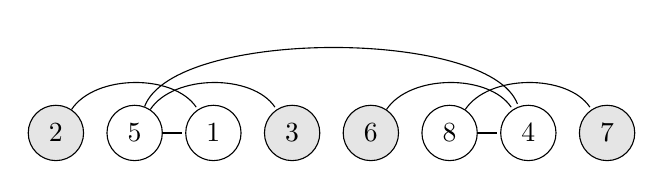
\begin{tikzpicture}[shorten >=1pt,-]
                \tikzstyle{vertex}=[circle,draw=black,fill=white!25,minimum size=20pt,inner sep=0pt]
                \tikzstyle{vertex2}=[circle,draw=black!,fill=black!10,minimum size=20pt,inner sep=0pt]
                \foreach \num/\x in {5/1, 1/2, 8/5, 4/6}
                        \node[vertex] (V-\num) at (\x,0) {$\num$};
                \foreach \num/\x in {2/0, 3/3, 6/4, 7/7}
                        \node[vertex2] (V-\num) at (\x,0) {$\num$};
            
                    \foreach \from/\to in {5/1, 8/4}
                        \draw (V-\from) -- (V-\to);
            
                    \draw (V-2) .. controls (0.5, 0.75) and (1.5, 0.75) .. (V-1);
                    \draw (V-6) .. controls (4.5, 0.75) and (5.5, 0.75) .. (V-4);
        
                    \draw (V-5) .. controls (1.5, 0.75) and (2.5, 0.75) .. (V-3);
                    \draw (V-8) .. controls (5.5, 0.75) and (6.5, 0.75) .. (V-7);
                    \draw (V-5) .. controls (1.5, 1.33) and (5.5, 1.33) .. (V-4);
            \end{tikzpicture}\\\quad\\                    
            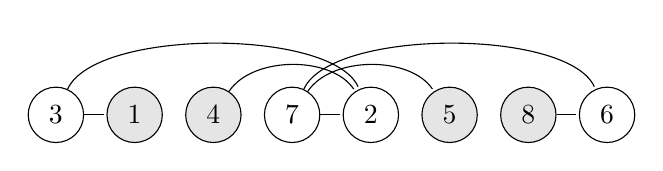
\begin{tikzpicture}[shorten >=1pt,-]
                \tikzstyle{vertex}=[circle,draw=black,fill=white!25,minimum size=20pt,inner sep=0pt]
                \tikzstyle{vertex2}=[circle,draw=black!,fill=black!10,minimum size=20pt,inner sep=0pt]
                \foreach \num/\x in {3/0, 7/3, 2/4, 6/7}
                        \node[vertex] (V-\num) at (\x,0) {$\num$};
                \foreach \num/\x in {1/1, 4/2, 5/5, 8/6}
                        \node[vertex2] (V-\num) at (\x,0) {$\num$};
            
                    \foreach \from/\to in {3/1, 7/2, 8/6}
                        \draw (V-\from) -- (V-\to);
            
                    \draw (V-4) .. controls (2.5, 0.75) and (3.5, 0.75) .. (V-2);
                    \draw (V-7) .. controls (3.5, 0.75) and (4.5, 0.75) .. (V-5);
    
                    \draw (V-3) .. controls (0.5, 1.1) and (3.5, 1.1) .. (V-2);
                    \draw (V-7) .. controls (3.5, 1.1) and (6.5, 1.1) .. (V-6);
            \end{tikzpicture}
        \end{center}
        \label{tranzitivni_orientaciji_gosenice}
    \end{figure}
}
% \frame{
%     % \frametitle{Odločitveno drevo}
%     \begin{figure}[h]
%         \begin{center}        
%             \begin{tikzpicture}[shorten >=1pt,-]
%                 \tikzstyle{vertex}=[circle,draw=black!0,fill=white!25,minimum size=20pt,inner sep=0pt]
%                 \tikzstyle{vertex2}=[circle,draw=black!0,fill=white!25,minimum size=0pt,inner sep=0pt]
                
%                 \node[vertex] (V-0) at (3.5, 8) {$\sigma$};
%                 \node[vertex] (V-11) at (-1, 7) {$\sigma_1$};
%                 \node[vertex] (V-22) at (-1, 6) {$\sigma_2$};
%                 \node[vertex] (V-33) at (-1, 5) {$\sigma_3$};
%                 \node[vertex] (V-44) at (-1, 4) {$\sigma_4$};
%                 \node[vertex] (V-55) at (-1, 3) {$\sigma_5$};
%                 % \node[vertex] (V-66) at (-1, 2) {$\sigma_6$};
%                 % \node[vertex] (V-77) at (-1, 1) {$\sigma_7$};
%                 \node[vertex2] (V-88) at (-1, 2.3) {};
%                 \node[vertex] (V-111) at (0.5, 7) {};
%                 \node[vertex] (V-222) at (0.5, 6) {};
%                 \node[vertex] (V-333) at (0.5, 5) {};
%                 \node[vertex] (V-444) at (0.5, 4) {};
%                 \node[vertex] (V-555) at (0.5, 3) {};
%                 % \node[vertex] (V-666) at (0.5, 2) {};
%                 % \node[vertex] (V-777) at (0.5, 1) {};
    
%                 \node[vertex] (V-12) at (3, 7) {$2$};
%                 \node[vertex] (V-23) at (2, 6) {$3$};
%                 \node[vertex] (V-24) at (3, 6) {$4$};
%                 \node[vertex] (V-31l) at (2, 5) {$1$};
%                 \node[vertex] (V-31d) at (3, 5) {$1$};
%                 \node[vertex] (V-45) at (2, 4) {$5$};
%                 \node[vertex] (V-43) at (1, 4) {$3$};
%                 \node[vertex] (V-46) at (3, 4) {$6$};
%                 \node[vertex] (V-53l) at (2, 3) {$3$};
%                 \node[vertex] (V-53d) at (3, 3) {$3$};
%                 % \node[vertex] (V-68) at (3, 2) {$8$};
%                 % \node[vertex] (V-67) at (2, 2) {$7$};
%                 % \node[vertex] (V-65) at (1, 2) {$5$};
%                 % \node[vertex] (V-75l) at (2, 1) {$5$};
%                 % \node[vertex] (V-75d) at (3, 1) {$5$};
%                 \node[vertex2] (V-80) at (3, 2.3) {};
%                 \node[vertex2] (V-800) at (2, 2.3) {};
%                 \node[vertex2] (V-8000) at (1, 2.3) {};
    
%                 \node[vertex] (V-13) at (4, 7) {$3$};
%                 \node[vertex] (V-21) at (4, 6) {$1$};
%                 \node[vertex] (V-35) at (4, 5) {$5$};
%                 \node[vertex] (V-34) at (5, 5) {$4$};
%                 \node[vertex] (V-32) at (6, 5) {$2$};
%                 \node[vertex] (V-42l) at (4, 4) {$2$};
%                 \node[vertex] (V-42d) at (5, 4) {$2$};
%                 % \node[vertex] (V-57) at (4, 3) {$7$};
%                 % \node[vertex] (V-56) at (5, 3) {$6$};
%                 % \node[vertex] (V-54) at (6, 3) {$4$};
%                 % \node[vertex] (V-64l) at (4, 2) {$4$};
%                 % \node[vertex] (V-64d) at (5, 2) {$4$};
%                 \node[vertex2] (V-70) at (4, 3.3) {};
%                 \node[vertex2] (V-700) at (5, 3.3) {};
%                 \node[vertex2] (V-7000) at (6, 3.3) {};
                
    
%                 \foreach \from/\to in {0/12, 0/13, 12/23, 12/24, 23/31l, 24/31d, 31d/43, 31d/45, 31d/46, 45/53l, 46/53d,
%                 13/21, 21/35, 21/34, 21/32, 35/42l, 34/42d}
%                     \draw (V-\from) -- (V-\to);
    
%                 \draw[dotted] (V-53d) -- (V-80);
%                 \draw[dotted] (V-53d) -- (V-800);
%                 \draw[dotted] (V-53d) -- (V-8000);
%                 \draw[dotted] (V-42l) -- (V-70);
%                 \draw[dotted] (V-42l) -- (V-700);
%                 \draw[dotted] (V-42l) -- (V-7000);            
%                 \draw[dotted] (V-55) -- (V-88);
    
%                 \foreach \from/\to in {11/111, 22/222, 33/333, 44/444, 55/555}
%                     \draw[-latex] (V-\from) -- (V-\to);
%                 \end{tikzpicture}     
%         \end{center}
%         \label{dve_permutaciji_poti}
%     \end{figure}
% }

%%%%%%%%%%%%%%%%%%%%%%%%%%%%%%%%%%%%%%%%%%%%%
\section{Tekmovalnostni grafi}
\frame{
    \frametitle{Rangiranja in tekmovalnost vozlišč}
    
    \begin{block}{Definicija rangiranja:}
        Rangiranje $c = (i_1, \dots, i_n)$ množice $[n]$ je permutacija iz $S_n$. Pisali bomo $i \prec_c j$, kadar se vozlišče $i$ pojavi pred vozliščem $j$ v vektorju rangiranja $c$.
    \end{block}
    \begin{block}{Definicija tekmovanja para vozlišč:}
        Naj bo $R = \{c_1, c_2, \dots, c_r\}$ končna množica rangiranj. Potem rečemo, da par vozlišč $(i, j) \in [n] \times [n]$ (neposredno) tekmuje, če obstajata takšni rangiranji $c_s, c_t \in R$, da je $i \prec_{c_s} j$ ampak $j \prec_{c_t} i$.
    \end{block}
    Naj bo $R = \{ c_1, c_2, c_3\}$ množica rangiranj množice $[6]$:
    \[
        c_1 = (1, 2, 3, 4, 5, 6), \quad c_2 = (2, 1, 3, 4, 6, 5), \quad c_3 = (1, 4, 2, 3, 5, 6).
    \]
    Pari vozlišč $(1, 2), (2, 4), (3, 4)$ in $(5, 6)$ tekmujejo.
}

\frame{
    \frametitle{Tekmovalnostni grafi}
    \begin{block}{Definicija tekmovanja para vozlišč:}
        Naj bo $R = \{ c_1, c_2, \dots, c_r \}$ množica rangiranj množice $[n]$. Tekmovalnostni graf množice rangiranj $R$ definiramo kot neusmerjen graf $G_c(R) = ([n], E)$, kjer je množica povezav $E$ podana na nasledni način: med $i$ in $j$ je povezava, če $(i, j)$ tekmujeta.
    \end{block}
    \begin{figure}[ht]
        \begin{center}
            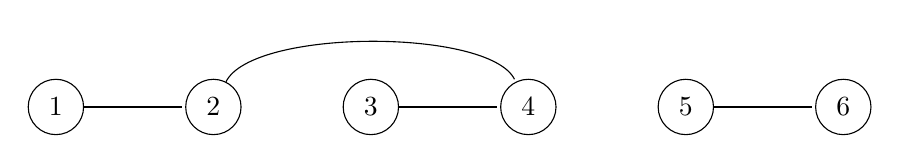
\begin{tikzpicture}[shorten >=1pt,-]
                \tikzstyle{vertex}=[circle,draw=black,fill=white!25,minimum size=20pt,inner sep=0pt]
                \foreach \num/\x in {1/1, 2/3, 3/5, 4/7, 5/9, 6/11}
                        \node[vertex] (V-\num) at (\x,0) {\num};
            
                    \foreach \from/\to in {1/2, 3/4, 5/6}
                        \draw (V-\from) -- (V-\to);
                    \draw (V-2) .. controls (3.5, 1) and (6.5, 1) .. (V-4);
            \end{tikzpicture}
        \end{center}
        \label{graf_tekmovalnosti_primer}
    \end{figure}
}
\frame{
    \frametitle{Delna kohezivnost}
    
    \begin{block}{Definicija delne kohezivnosti:}
        % Graf $G$ ima  delno kohezivno zaporedje, če obstaja povezava $ab$, kjer $a < b$, potem mora za vsak $x$, za katerega velja $a < x < b$ obstajati povezava $ax$ ali $xb$. Graf $G$ je delno koheziven, če ima delno kohezivno zaporedje.

        Naj bo $G$ neusmerjen graf na $n$ vozliščih. 
        Zaporedju vozlišč $l = (v_1, v_2, \dots, v_n)$ rečemo delno kohezivno zaporedje grafa $G$, če za poljubne $i, j, k$, kjer je $1 \leq i < k < j \leq n$ velja naslednji pogoj:
        \begin{enumerate}[label=(b)]
            \item Če je $v_iv_j \in E(G)$, potem je $v_iv_k \in E(G)$ ali $v_kv_j \in E(G)$.
        \end{enumerate}
        Graf $G$ je delno koheziven, če ima delno kohezivno zaporedje.        
    \end{block}
    \begin{block}{Izrek:}
        Vsak tekmovalnostni graf je delno koheziven.
    \end{block}
}
\frame{
    \frametitle{Množice posrednih in neposrednih tekmovalcev}
    
    % \begin{block}{Definicija množice tekmovalcev:}
    %     Naj bo $R = \{ c_1, c_2, \dots, c_r\}$ množica rangiranj množice $[n]$. Množici  vozlišč $C \subseteq [n]$ rečemo množica tekmovalcev, če vsaka dva elementa $i, j \in C$ tekmujeta in $C$ je maksimalna glede na to lastnost.
    % \end{block}
    \begin{block}{Definicija množice posrednih in neposrednih tekmovalcev:}
        Če vzamemo množico rangiranj $R = \{ c_1, \dots, c_r\}$ množice $[n]$, rečemo, da par vozlišč $(i, j) \in [n] \times [n]$ posredno ali neposredno tekmuje, če obstaja tak $k \in \mathbb{N}$ in vozlišča $i_1, \dots, i_k \in [n]$, da $(i, i_1)$ tekmujeta, $(i_1, i_2)$ tekmujeta, $\dots$, in $(i_k, j)$ tekmujeta.
    
        Množici vozlišč $D \subseteq [n]$ rečemo množica posrednih in neposrednih tekmovalcev, če vsaka dva elementa $i, j \in D$ posredno ali neposredno tekmujeta in $D$ je maksimalna glede na to lastnost.
    \end{block}
    \begin{figure}[ht]
        \begin{center}
            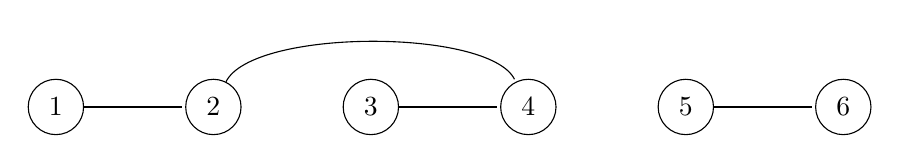
\begin{tikzpicture}[shorten >=1pt,-]
                \tikzstyle{vertex}=[circle,draw=black,fill=white!25,minimum size=20pt,inner sep=0pt]
                \foreach \num/\x in {1/1, 2/3, 3/5, 4/7, 5/9, 6/11}
                        \node[vertex] (V-\num) at (\x,0) {\num};
            
                    \foreach \from/\to in {1/2, 3/4, 5/6}
                        \draw (V-\from) -- (V-\to);
                    \draw (V-2) .. controls (3.5, 1) and (6.5, 1) .. (V-4);
            \end{tikzpicture}
        \end{center}
        \label{graf_tekmovalnosti_primer2}
    \end{figure}
}
\frame{
    \frametitle{Algoritem za izračun množic posrednih in neposrednih tekmovalcev}
    \[
        D_{[p, q]} = \{ x \in [n] \ | \ c_s^{-1}(x) \in [p, q] \ za \ nek \ c_s \in R\}
    \]
    \begin{align}
        c_1 = (1, 2, 3, 4, 5, 6) \notag\\
        c_2 = (2, 1, 3, 4, 6, 5) \notag\\
        c_3 = (1, 4, 2, 3, 5, 6) \notag
    \end{align}
    \begin{align}
        D_{[1,1]} &=  \{ 1, 2 \} \subseteq D_1 & &max\{ 1, 2, 3\} = 3\notag\\
        D_{[1,3]} &= \{ 1, 2, 3, 4\} \subseteq D_1 & &max\{ 1, 2, 3, 4\} = 4 \notag\\
        D_{[1,4]} &= \{ 1, 2, 3, 4\} = D_1 \notag\\
        D_{[5,5]} &= \{ 5, 6 \} \subseteq D_2 & &max\{ 5, 6\} = 6 \notag\\
        D_{[5,6]} &= \{ 5, 6\} = D_2 \notag
    \end{align}
    % \begin{figure}[ht]
    %     \begin{center}
    %         \begin{tikzpicture}[shorten >=1pt,-]
    %             \tikzstyle{vertex}=[circle,draw=black,fill=white!25,minimum size=20pt,inner sep=0pt]
    %             \foreach \num/\x in {1/1, 2/3, 3/5, 4/7, 5/9, 6/11}
    %                     \node[vertex] (V-\num) at (\x,0) {\num};
            
    %                 \foreach \from/\to in {1/2, 3/4, 5/6}
    %                     \draw (V-\from) -- (V-\to);
    %                 \draw (V-2) .. controls (3.5, 1) and (6.5, 1) .. (V-4);
    %         \end{tikzpicture}
    %     \end{center}
    %     \label{graf_tekmovalnosti_primer3}
    % \end{figure}
}
%%%%%%%%%%%%%%%%%%%%%%%%%%%%%%%%%%%%%%%%%%%%%
\section{Zaključek}
\frame{
    \frametitle{Zaključek}
    Pogledali smo si, kaj so inverzije permutacij, njihove lastnosti in kako definirajo permutacijske in tekmovalnostne grafe.

    Permutacijske grafe smo karakterizirali s kohezivnim zaporedjem. Povedali smo, da so gosenice edina drevesa, ki so permutacijski grafi, in da obstajata natanko dve permutaciji iz $S_n$, ki imata permutacijski graf izomorfen neki gosenici na $n \geq 3$ vozliščih.
    
    Potem smo definirali, kaj so rangiranja, kdaj par vozlišč tekmuje ter kaj je množica posrednih in neposrednih tekmovalcev.  Pogledali smo si, kaj so tekmovalnostni grafi in povedali, da so delno kohezivni. Na koncu smo predstavili algoritem za izračun množic posrednih in neposrednih tekmovalcev.
}
% \frame{
%     \frametitle{Lemi}

%     \begin{block}{Lema:}
%         Naj bo $R = \{ c_1, \dots, c_r \}$ množica rangiranj množice $[n]$. Če je $D \subseteq [n]$ množica posrednih in neposrednih tekmovalcev in $a, b \in D$, potem za vsak $x \in [n]$ in vsako tako rangiranje $c_m \in R$, da je $a \prec_{c_m} x \prec_{c_m} b$, sledi $x \in D$.
%     \end{block}
%     \begin{block}{Lema:}
%         Naj bo $R = \{ c_1, \dots, c_r \}$ množica rangiranj množice $[n]$. Če je $D \subseteq [n]$ množica posrednih in neposrednih tekmovalcev ter obstajata taka $a \in D$ in  $c_m \in R$, da je $c_m^{-1}(a) = 1$, potem 
%         \[
%             \{ x \in [n] \ | \ c_s^{-1}(x) = 1 \ za \ nek \ c_s \in R \} \subseteq D.    
%         \]
%         % To pomeni, da vsi elementi na prvi poziciji rangiranj iz $R$ pripadajo $D$.
%     \end{block}
% }
% \frame{
%     \frametitle{Algoritem za izračun množice posrednih in neposrednih tekmovalcev}
    
%     \begin{block}{Izrek:}
%         Naj bo $R = \{ c_1, \dots, c_r \}$ množica rangiranj vozlišč $[n]$. Množico posrednih in neposrednih tekmovalcev lahko identificiramo z zaprtimi intervali naravnih števil $[p, q]$ na naslednji način: 
%         \[
%             D_{[p, q]} = \{ x \in [n] \ | \ c_s^{-1}(x) \in [p, q] \ za \ nek \ c_s \in R\}.
%         \]
%         Še več, $p$ in $q$ sta prvi na levi in zadnji na desni poziciji elementov iz $D_{[p, q]}$ glede na vsa rangiranja.
%     \end{block}
% }
% \frame{
%     \frametitle{Usmerjen graf $G_d(R)$}
    
%     \begin{block}{Definicija usmerjenega grafa $G_d(R)$:}
%         Naj bo $R = \{ c_1, \dots, c_r \}$ množica $r$ rangiranj $(r \geq 2)$ množice $[n]$. Definirajmo usmerjen graf $G_d(R)$  na naslednji način:
%         \begin{enumerate}[label=(\roman*)]
%             \item Vozlišča grafa $G_d(R)$ so elementi množice $[n]$.
%             \item Če $i, j \in [n]$, $i \neq j$ potem je $(i, j)$ usmerjena povezava v grafu $G_d(R)$, če obstaja takšno rangiranje $c_m \in R$, da je $i \preceq_{c_m} j$.
%         \end{enumerate}
%     \end{block}
% }
% \frame{
%     \frametitle{Ekvivalentnost trditev o usmerjenem grafu $G_d(R)$}
    
%     \begin{block}{Trditev:}
%         Naj bosta $D_1$ in $D_2$ dve različni množici posrednih in neposrednih tekmovalcev. Naslednji trditvi o usmerjenem grafu $G_d(R)$ sta ekvivalentni:
%         \begin{enumerate}[label=(\roman*)]
%             \item Obstaja takšna usmerjena povezava $(a, b)$, da je $a \in D_1$ in $b \in D_2$.
%             \item Vsa vozlišča iz $D_1$ imajo usmerjeno povezavo proti vsem vozliščem iz $D_2$.
%         \end{enumerate}
%     \end{block}
% }
% \frame{
%     \frametitle{Relacija $\rightarrow$}
    
%     \begin{block}{Definicija relacije $\rightarrow$:}
%         Naj bo $R = \{ c_1, \dots, c_r \}$ množica r rangiranj vozlišč $[n]$, $r \geq 2$, katerih množice posrednih in neposrednih tekmovalcev označimo z $D_1, \dots, D_k$, kjer je$\underset{i \in [k]}{\cup} D_i = [n]$. Definirajmo binarno relacijo $\rightarrow$ med dvema množicama posrednih in neposrednih tekmovalcev na nasledni način:
%         \begin{enumerate}[label=(\roman*)]
%             \item $D_i \rightarrow D_i$ za vsako množico posrednih in neposrednih tekmovalcev $D_i$.
%             \item za vsaki različni množici $D_i, D_j$ posrednih in neposrednih tekmovalcev, je $D_i \rightarrow D_j$ natanko tedaj, ko velja katerakoli od ekvivalentnih trditev o usmerjenem grafu $G_d(R)$ iz prejšne trditve.
%         \end{enumerate}
%     \end{block}
% }
% \frame{
%     \frametitle{Latnosti relacije $\rightarrow$}
    
%     \begin{block}{Lema:}
%         Binarna relacija $\rightarrow$ je tranzitivna.
%     \end{block}
%     \begin{block}{Posledica:}
%         Binarna relacija $\rightarrow$ je linearna urejenost množic posrednih in neposrednih tekmovalcev iz $[n]$.
%     \end{block}
% }

\end{document}